\upaper{11}{ВЕЧНЫЙ ОСТРОВ РАЙ}
\uminitoc{БОЖЕСТВЕННАЯ РЕЗИДЕНЦИЯ}
\uminitoc{ПРИРОДА ВЕЧНОГО ОСТРОВА}
\uminitoc{ВЕРХНИЙ РАЙ}
\uminitoc{ПЕРИФЕРИЙНЫЙ РАЙ}
\uminitoc{НИЖНИЙ РАЙ}
\uminitoc{ДЫХАНИЕ ПРОСТРАНСТВА}
\uminitoc{ПРОСТРАНСТВЕННЫЕ ФУНКЦИИ РАЯ}
\uminitoc{ГРАВИТАЦИЯ РАЯ}
\uminitoc{УНИКАЛЬНОСТЬ РАЯ}
\author{Совершенствователь Мудрости}
\vs p011 0:1 Рай --- вечный центр вселенной вселенных и место пребывания Всеобщего Отца, Вечного Сына, Бесконечного Духа и их божественных равных и партнёров. Этот центральный Остров представляет собой самое гигантское организованное тело космической реальности во всей главной вселенной. Рай --- это как материальная сфера, так и духовная обитель. Всё разумное творение Всеобщего Отца расселено на материальных местах обитания; поэтому и абсолютный управляющий центр должен быть также материальным, буквальным. И вновь необходимо повторить, что предметы духа и духовные существа \bibemph{реальны}.
\vs p011 0:2 Материальная красота Рая состоит в великолепии его физического совершенства; величие Острова Бога представлено в возвышенных интеллектуальных достижениях и развитии разума его обитателей; слава центрального Острова явлена в бесконечном даровании божественной личности духа --- свете жизни. Но глуб\'ины духовной красоты и чудеса этого великолепного ансамбля совершенно за пределами понимания конечного разума материальных созданий. Слава и духовное великолепие божественной обители недоступны смертному пониманию. И Рай --- от вечности; нет ни записей, ни преданий относительно происхождения этого центрального ядра --- Острова Света и Жизни.
\usection{БОЖЕСТВЕННАЯ РЕЗИДЕНЦИЯ}
\vs p011 1:1 Рай служит многим целям в управлении вселенскими сферами, но для созданий он существует прежде всего как место обитания Божества. Личное присутствие Всеобщего Отца расположено в самом центре верхней поверхности этой почти круглой, но не сферической обители Божеств. Это Райское присутствие Всеобщего Отца непосредственно окружено личным присутствием Вечного Сына, в то время как оба они окутаны несказ\'анной славой Бесконечного Духа.
\vs p011 1:2 Бог обитает, обитал и всегда будет обитать в этой центральной и вечной обители. Мы всегда находили и всегда будем находить его там. Всеобщий Отец космически фокализован, духовно персонализован и географически постоянно присутствует в этом центре вселенной вселенных.
\vs p011 1:3 \pc Мы все знаем прямой путь, по которому надо следовать, чтобы найти Всеобщего Отца. Ты не способен постичь многого относительно божественной резиденции из\hyp{}за её удалённости от тебя и необъятности пролегающего пространства, но те, кто способен понять значение этих огромных расстояний, знают положение и место жительства Бога так же определённо и буквально, как ты знаешь местоположение Нью\hyp{}Йорка, Лондона, Рима или Сингапура --- городов, определённо и географически расположенных на Урантии. Если ты знающий штурман, оснащённый кораблём, картами и компасом, ты сможешь легко найти эти города. Точно так же, если бы ты располагал временем и средствами передвижения, имел достаточную духовную подготовку и необходимое указание направления, ты мог бы проходить от вселенной к вселенной и от контура к контуру, постоянно продвигаясь внутрь через звёздные миры, пока, наконец, не предстал бы перед центральным сиянием духовной славы Всеобщего Отца. Предусмотрев всё необходимое для путешествия, так же возможно найти личное присутствие Бога в центре всего сущего, как найти далёкие города на твоей собственной планете. То, что ты не посещал эти места, нисколько не опровергает их реальность или актуальность их существования. То, что так мало вселенских созданий нашли Бога на Рае, ни в коей мере не опровергает ни реальности его существования, ни актуальности его духовного лица в центре всего сущего.
\vs p011 1:4 Отца всегда можно найти в этом центральном месте. Если бы он переместился, возник бы всеобщий хаос, ибо в нём, в центре его обитания, сходятся всеобщие линии гравитации со всех концов творения. Отслеживаем ли мы личностный контур обратно к вселенным или следуем за восходящими личностями, когда они путешествуют внутрь к Отцу; отслеживаем ли мы линии материальной гравитации к нижнему Раю или следуем за циклическими всплесками космической силы; отслеживаем ли мы линии духовной гравитации к Вечному Сыну или следуем за продвигающейся вовнутрь процессией Райских Сынов Бога; прослеживаем ли мы контуры разума или следуем за триллионами и триллионами небесных существ, которые происходят от Бесконечного Духа, --- любое из этих наблюдений или все они приводят нас непосредственно к присутствию Отца, к его центральной обители. Здесь Бог присутствует лично, буквально и актуально. И от его бесконечного существа изливаются реки\hyp{}потоки жизни, энергии и личности для всех вселенных.
\usection{ПРИРОДА ВЕЧНОГО ОСТРОВА}
\vs p011 2:1 Так как ты уже начинаешь осознавать громадность материальной вселенной, различимую даже из вашего астрономического местонахождения, вашего положения в пространстве в звёздных системах, тебе должно становиться очевидным, что такая огромная материальная вселенная должна иметь соответствующую и достойную столицу, центр, соразмерный достоинству и бесконечности всеобщего Правителя всего этого громадного и далеко раскинувшегося творения материальных миров и живых существ.
\vs p011 2:2 \pc По форме Рай отличается от обитаемых космических тел: он не сферический. Это определённо эллипсоид, на одну шестую длиннее в диаметре в направлении север\hyp{}юг, чем в диаметре восток\hyp{}запад. Центральный Остров практически плоский: расстояние от верхней поверхности до нижней поверхности составляет одну десятую диаметра в направлении восток\hyp{}запад.
\vs p011 2:3 Эти различия в размерах, взятые в связи с его стационарным статусом и б\'ольшим исходящим давлением силы\hyp{}энергии на северном конце Острова, позволяют установить абсолютное направление в главной вселенной.
\vs p011 2:4 \pc Центральный Остров географически разделён на три области активности:
\vs p011 2:5 \li{1.}Верхний Рай.
\vs p011 2:6 \li{2.}Периферийный Рай.
\vs p011 2:7 \li{3.}Нижний Рай.
\vs p011 2:8 \pc Мы называем поверхность Рая, занятую личностной деятельностью, --- верхней стороной, а противоположную поверхность --- нижней стороной. Периферия Рая предназначена для деятельности, которая не является в строгом смысле личностной или неличностной. Троица, по\hyp{}видимому, доминирует на личностной, или верхней, плоскости; Безусловный Абсолют --- на нижней, или неличностной, плоскости. Мы вряд ли представляем себе Безусловный Абсолют как личность, но мы действительно думаем, что функциональное пространственное присутствие этого Абсолюта сосредоточено на нижнем Рае.
\vs p011 2:9 \pc Вечный Остров состоит из единственной формы материализации --- стационарных систем реальности. Эта буквальная субстанция Рая представляет собой однородную организацию потенции пространства, которую нельзя найти где\hyp{}либо ещё во всей обширной вселенной вселенных. Она получила многочисленные названия в различных вселенных, и Мелхиседеки Небадона давно назвали её \bibemph{абсолютум}. Этот исходный материал Рая не является ни мёртвым, ни живым; это --- изначальное недуховное выражение Первого Источника и Центра; это --- Рай, а Рай не имеет дубликатов.
\vs p011 2:10 Нам представляется, что Первый Источник и Центр сконцентрировал весь абсолютный потенциал для космической реальности в Раю как часть своего метода самоосвобождения от ограничений бесконечности, как средство создания возможности суббесконечного, даже время\hyp{}пространственного, творения. Но из этого не следует, что Рай ограничен во времени и пространстве только потому, что вселенная вселенных раскрывает эти качества. Рай существует вне времени и не имеет положения в пространстве.
\vs p011 2:11 Ориентировочно: пространство, по\hyp{}видимому, возникает сразу же под нижним Раем; время --- сразу же над верхним Раем. Время, как вы его понимаете, не является характерной чертой Райского существования, хотя жители центрального Острова полностью осознают вневременн\'ую последовательность событий. Движение не является необходимостью на Рае, оно --- следствие волеизъявления. Но концепция расстояния, даже абсолютного расстояния, имеет очень большое значение, ибо оно может применяться к относительным местоположениям на Рае. Рай внепространственен, поэтому его области абсолютны и, следовательно, могут использоваться многими способами, выходящими за рамки концепций смертного разума.
\usection{ВЕРХНИЙ РАЙ}
\vs p011 3:1 На верхнем Рае расположены три большие области деятельности: \bibemph{присутствие Божества,} \bibemph{Святейшая Сфера} и \bibemph{Святая Область}. Обширный регион, непосредственно окружающий присутствие Божеств, выделен как Святейшая Сфера и отведён для функций поклонения, тринитизации и высокого духовного достижения. В этой зоне нет ни материальных структур, ни чисто интеллектуальных творений; они не могли бы там существовать. Мне бесполезно пытаться описать человеческому разуму божественную природу и прекрасное величие Святейшей Сферы Рая. Эта область целиком духовна, а ты почти целиком материален. Для чисто материального существа чисто духовная реальность как будто не существует.
\vs p011 3:2 Хотя в Святейшей Сфере отсутствуют физические материализации, в секторах Святой Земли есть изобилие памятных свидетельств ваших материальных дней, и ещё больше в вызывающих воспоминания исторических областях периферийного Рая.
\vs p011 3:3 Святая Область --- внешний, или жилой, район --- разделена на семь концентрических зон. Рай иногда называют <<Домом Отца>>, ибо это его вечная резиденция, а эти семь зон часто называют <<Райскими обителями Отца>>. Внутреннюю, или первую, зону занимают Граждане Рая и уроженцы Хавоны, которым случается жить на Рае. Следующая, или вторая, зона --- это область обитания уроженцев семи сверхвселенных времени и пространства. Эта вторая зона частично поделена ещё на семь огромных разделов --- Райский дом духовных существ и восходящих созданий, происходящих из вселенных эволюционного развития. Каждый из этих секторов специально посвящён благополучию и развитию личностей отдельной сверхвселенной, но эти возможности почти бесконечно превышают потребности нынешних семи сверхвселенных.
\vs p011 3:4 Каждый из семи секторов Рая разделён на жилые единицы, предназначенные в качестве жилых центров для миллиарда рабочих групп прославленных индивидуумов. \begin{itemize}\item 1000 таких единиц составляет отделение. \item 100\,000 отделений равны одной конгрегации. \item 10\,000\,000 конгрегаций составляет ассамблею. \item 1\,000\,000\,000 ассамблей образует одну большую единицу.\end{itemize} И эта восходящая серия продолжается через вторую большую единицу, через третью и так далее --- до седьмой большой единицы. И семь больших единиц составляют главные единицы, и семь главных единиц образуют высшую единицу; и так --- кратно семи --- восходящий ряд расширяется через высшую, сверхвысшую, небесную, сверхнебесную до верховных единиц. Но даже и при этом не используется всё имеющееся в распоряжении пространство. Это ошеломляющее число жилых помещений на Рае --- число, выходящее за пределы твоего представления, --- занимает значительно меньше 1\% отведённой области Святой Земли. Ещё остаётся предостаточно места для тех, кто находится на своём пути внутрь, и даже для тех, кто не начнёт восхождение к Раю до наступления времён вечного будущего.
\usection{ПЕРИФЕРИЙНЫЙ РАЙ}
\vs p011 4:1 Центральный Остров резко обрывается на периферии, но его размер настолько огромен, что этот крайний угол относительно неразличим в пределах любой ограниченной области. Периферийная поверхность Рая частично занята взлётно\hyp{}посадочными площадками для различных групп духовных личностей. Поскольку зоны ненасыщенного пространства почти соприкасаются с периферией, весь личностный транспорт, направляющийся к Раю, производит посадку в этих регионах. Ни верхний, ни нижний Рай не доступны для транспортных супернафимов или других типов путешественников космоса.
\vs p011 4:2 Семь Главных Духов восседают каждый на своём троне могущества и власти на семи сферах Духа, обращающихся вокруг Рая в пространстве между сияющими сферами Сына и внутренним контуром миров Хавоны, но они сохраняют центры фокализации силы на периферии Рая. Здесь медленно циркулирующие присутствия Семи Верховных Управляющих Мощью указывают расположение семи станций, вспышками отправляющих в семь сверхвселенных определённые виды энергии Рая.
\vs p011 4:3 Здесь же, на периферии Рая, находятся колоссальные исторические и пророческие выставочные области, предназначенные для Сынов Создателей, посвящённые локальным вселенным времени и пространства. Существует ровно семь триллионов\fnst{Это максимальное число обитаемых планет в семи сверхвселенных.} таких исторических заповедников, ныне действующих или находящихся в резерве, но всё это устройство в совокупности занимает лишь около 4\% отведённой для этой цели части периферийной области. Мы предполагаем, что эти огромные резервы соответствуют творениям, которые когда\hyp{}нибудь появятся за пределами известных в настоящее время и обитаемых семи сверхвселенных.
\vs p011 4:4 Часть Рая, предназначенная для нужд существующих вселенных, занимает всего 1\%--4\%, в то время как отведённая для этой деятельности область по крайней мере в миллион раз превышает требуемую для подобных целей. Рай достаточно велик, чтобы вместить деятельность почти бесконечного творения.
\vs p011 4:5 Но дальнейшая попытка помочь тебе представить величие Рая будет тщетной. Ты должен подождать, и пока ожидаешь, продолжать своё восхождение, ибо истинно сказано: <<Глаз не видел, ухо не слышало, и не приходило на ум смертному человеку, чт\'о Всеобщий Отец приготовил для тех, кто переживёт жизнь во плоти на мирах времени и пространства>>.
\usection{НИЖНИЙ РАЙ}
\vs p011 5:1 О нижнем Рае мы знаем только то, что раскрыто; личности там не обитают. Он не имеет никакого отношения к делам разумных духов, не функционирует там и Божество Абсолют. Нам сообщают, что все контуры физической энергии и космической силы берут своё начало на нижнем Рае, и что он устроен следующим образом:
\vs p011 5:2 \li{1.}Прямо под месторасположением Троицы, в центральной части нижнего Рая, находится неизвестная и нераскрытая Зона Бесконечности.
\vs p011 5:3 \li{2.}Эта Зона непосредственно окружена безымянной областью.
\vs p011 5:4 \li{3.}Внешние границы нижней поверхности занимает область, в основном имеющая отношение к потенции пространства и силе\hyp{}энергии. Действие этого огромного эллиптического силового центра не идентифицируется с известными функциями какого\hyp{}либо триединства, но изначальный сила\hyp{}заряд пространства, по\hyp{}видимому, сосредоточен в этой области. Этот центр состоит из трёх концентрических эллиптических зон: самая внутренняя представляет собой фокальную точку энерго\hyp{}силовой деятельности самог\'о Рая; самая внешняя может быть идентифицирована с функциями Безусловного Абсолюта, но мы не знаем ничего определённого относительно пространственных функций средней зоны.
\vs p011 5:5 \pc Действие \bibemph{внутренней зоны} этого силового центра похоже на гигантское сердце, чьи пульсации направляют потоки энергии к самым внешним границам физического пространства. Она направляет и видоизменяет силы\hyp{}энергии, но вряд ли управляет их движением. Реальность давления\hyp{}присутствия этой изначальной силы определённо больше на северном конце Райского центра, чем в южных регионах; это различие регистрируется равномерно. Материнская сила пространства, по\hyp{}видимому, втекает на юге и вытекает на севере благодаря действию какой\hyp{}то неизвестной системы циркуляции, связанной с распространением этой основной формы силы\hyp{}энергии. Время от времени отмечаются также различия в давлениях по направлению восток\hyp{}запад. Силы, исходящие из этой зоны, не реагируют на наблюдаемую физическую гравитацию, но всегда подчиняются Райской гравитации.
\vs p011 5:6 \pc \bibemph{Средняя зона} силового центра непосредственно окружает эту область. Эта средняя зона кажется статичной, за исключением того, что она расширяется и сжимается, проходя три цикла активности. Наименьшая из этих пульсаций происходит в направлении восток\hyp{}запад , следующая --- в направлении север\hyp{}юг, тогда как наибольшие колебания --- общее расширение и сжатие --- происходят по всем направлениям. Функция этой средней области никогда не была полностью определена, но она должна иметь какое\hyp{}то отношение к взаимному регулированию между внутренней и внешней зонами силового центра. Многие считают, что средняя зона --- это механизм управления промежуточным пространством или зонами покоя, которые разделяют последовательные пространственные уровни главной вселенной, но никакие доказательства или откровения не подтверждают это. Этот вывод основан на знании того, что эта средняя область каким\hyp{}то образом связана с функционированием механизма ненасыщенного пространства главной вселенной.
\vs p011 5:7 \pc \bibemph{Внешняя зона} --- самый большой и наиболее активный из трёх концентрических эллиптических поясов неидентифицированного потенциала пространства. Эта область --- арена невообразимой активности, центральная точка контуров, излучения которых отправляются в пространство по всем направлениям к самым внешним границам семи сверхвселенных и дальше, охватывая огромные и непостижимые области всего внешнего пространства. Это пространственное присутствие полностью безличностно, несмотря на то, что каким\hyp{}то нераскрытым образом оно, по\hyp{}видимому, косвенно реагирует на волю и распоряжения бесконечных Божеств, действующих в качестве Троицы. Считается, что здесь сфокусирован Райский центр пространственного присутствия Безусловного Абсолюта.
\vs p011 5:8 Все формы силы и все фазы энергии, по\hyp{}видимому, замкнуты в контуры; они циркулируют по вселенным и возвращаются определёнными путями. Но излучения активированной зоны Безусловного Абсолюта, по\hyp{}видимому, либо исходящие, либо входящие, --- никогда оба действия не происходят одновременно. Эта внешняя зона пульсирует циклами гигантских размеров эпохальной протяжённости. В течение чуть более миллиарда лет Урантии пространство\hyp{}сила этого центра исходит наружу; затем в течение аналогичного промежутка времени она возвращается вовнутрь. И проявления пространства\hyp{}силы этого центра универсальны; они распространяются по всему насыщенному пространству.
\vs p011 5:9 \pc Вся физическая сила, энергия и материя едины. Вся сила\hyp{}энергия первоначально исходит из нижнего Рая и в конечном итоге вернётся туда после прохождения своего пространственного контура. Но не все виды энергии и материальной организации вселенной вселенных вышли из нижнего Рая в их современных видимых состояниях; пространство --- это лоно нескольких форм материи и предматерии. Хотя внешняя зона силового центра Рая является источником энергий пространства, само пространство там не возникает. Пространство --- это не сила, энергия или мощь. И пульсации этой зоны не являются причиной дыхания пространства, но чередование входящих и исходящих фаз этой зоны синхронизировано с циклами расширения\hyp{}сжатия пространства длительностью в два миллиарда лет.
\usection{ДЫХАНИЕ ПРОСТРАНСТВА}
\vs p011 6:1 Мы не знаем действительного механизма дыхания пространства; мы просто наблюдаем, что всё пространство попеременно сжимается и расширяется. Это дыхание влияет как на горизонтальную протяжённость насыщенного пространства, так и на вертикальную протяжённость ненасыщенного пространства, существующих в огромных резервуарах пространства выше и ниже Рая. Чтобы представить объёмные очертания этих резервуаров пространства, вспомни песочные часы.
\vs p011 6:2 В то время как вселенные горизонтального протяжения насыщенного пространства расширяются, резервуары вертикального протяжения ненасыщенного пространства сжимаются --- и наоборот. Непосредственно под нижним Раем происходит слияние насыщенного и ненасыщенного пространства. Оба типа пространства протекают там через преобразующие каналы регулирования, где при циклических сжатиях и расширениях космоса происходят изменения, делающие насыщаемое пространство ненасыщаемым, и наоборот.
\vs p011 6:3 \pc <<Ненасыщенным>> называется пространство, не пронизанное теми силами, энергиями, мощью и присутствиями, которые, как известно, существуют в насыщенном пространстве. Мы не знаем, предназначено ли вертикальное (резервуарное) пространство всегда служить противовесом горизонтальному (вселенскому) пространству; мы не знаем, существует ли творческий замысел в отношении ненасыщенного пространства; мы действительно очень мало знаем о резервуарах пространства --- только то, что они существуют, и что они, по\hyp{}видимому, уравновешивают циклы расширения\hyp{}сжатия пространства вселенной вселенных.
\vs p011 6:4 \pc Каждая фаза цикла дыхания пространства длится немногим более одного миллиарда лет Урантии. В течение одной фазы вселенные расширяются, в течение следующей --- сжимаются. В настоящее время насыщенное пространство подходит к средней точке фазы расширения, в то время как ненасыщенное пространство подходит к средней точке фазы сжатия, и нам известно, что наиболее удалённые границы обоих протяжений пространства, теоретически, сейчас приблизительно равноудалены от Рая. В настоящее время резервуары ненасыщенного пространства простираются по вертикали над верхним Раем и под нижним Раем на такое же расстояние, на какое насыщенное пространство вселенной простирается горизонтально наружу от периферийного Рая до четвёртого внешнего пространственного уровня и даже за его пределы.
\vs p011 6:5 В течение миллиарда лет времени Урантии резервуары пространства сжимаются, в то время как главная вселенная и силовая активность всего горизонтального пространства расширяются. Таким образом, для завершения полного цикла расширения\hyp{}сжатия требуется немногим более двух миллиардов лет Урантии.
\usection{ПРОСТРАНСТВЕННЫЕ ФУНКЦИИ РАЯ}
\vs p011 7:1 Пространство не существует ни на одной из поверхностей Рая. Если <<посмотреть>> прямо вверх с верхней поверхности Рая, то не <<увидишь>> ничего, кроме ненасыщенного пространства, исходящего или входящего, в настоящее время --- входящего. Пространство не касается Рая; только спокойные \bibemph{зоны промежуточного пространства} соприкасаются с центральным Островом.
\vs p011 7:2 Рай --- это фактически неподвижное ядро относительно спокойных зон, существующих между насыщенным и ненасыщенным пространством. Географически эти зоны кажутся относительным продолжением Рая, но в них, вероятно, существует какое\hyp{}то движение. Мы знаем о них очень мало, но мы наблюдаем, что эти зоны уменьшённого пространственного движения разделяют насыщенное и ненасыщенное пространства. Подобные зоны существовали когда\hyp{}то между уровнями насыщенного пространства, но сейчас они менее спокойны.
\vs p011 7:3 Вертикальное поперечное сечение всего пространства немного напоминает мальтийский крест, где горизонтальные протяжённости представляют насыщенное (вселенское) пространство, и вертикальные --- ненасыщенное (резервуарное) пространство. Области между четырьмя протяжённостями разделены подобно тому, как зоны промежуточного пространства разделяют насыщенное и ненасыщенное пространство. Эти спокойные зоны промежуточного пространства становятся всё больше и больше по мере удаления от Рая и в итоге охватывают границы всего пространства, полностью включая в себя как резервуары пространства, так и всю горизонтальную протяжённость насыщенного пространства.
\vs p011 7:4 \pc Пространство не является ни субабсолютным состоянием внутри Безусловного Абсолюта, ни его присутствием, ни функцией Предельного. Это --- дар Рая, и считается, что пространство большой вселенной и всех внешних областей на самом деле насыщено изначальной пространственной потенцией Безусловного Абсолюта. От непосредственно примыкающих к периферийному Раю областей это насыщенное пространство простирается горизонтально наружу через четвёртый пространственный уровень и выходит за пределы периферии главной вселенной, но как далеко, мы не знаем.\tunemarkup{pictures}{\begin{figure}[H]\centering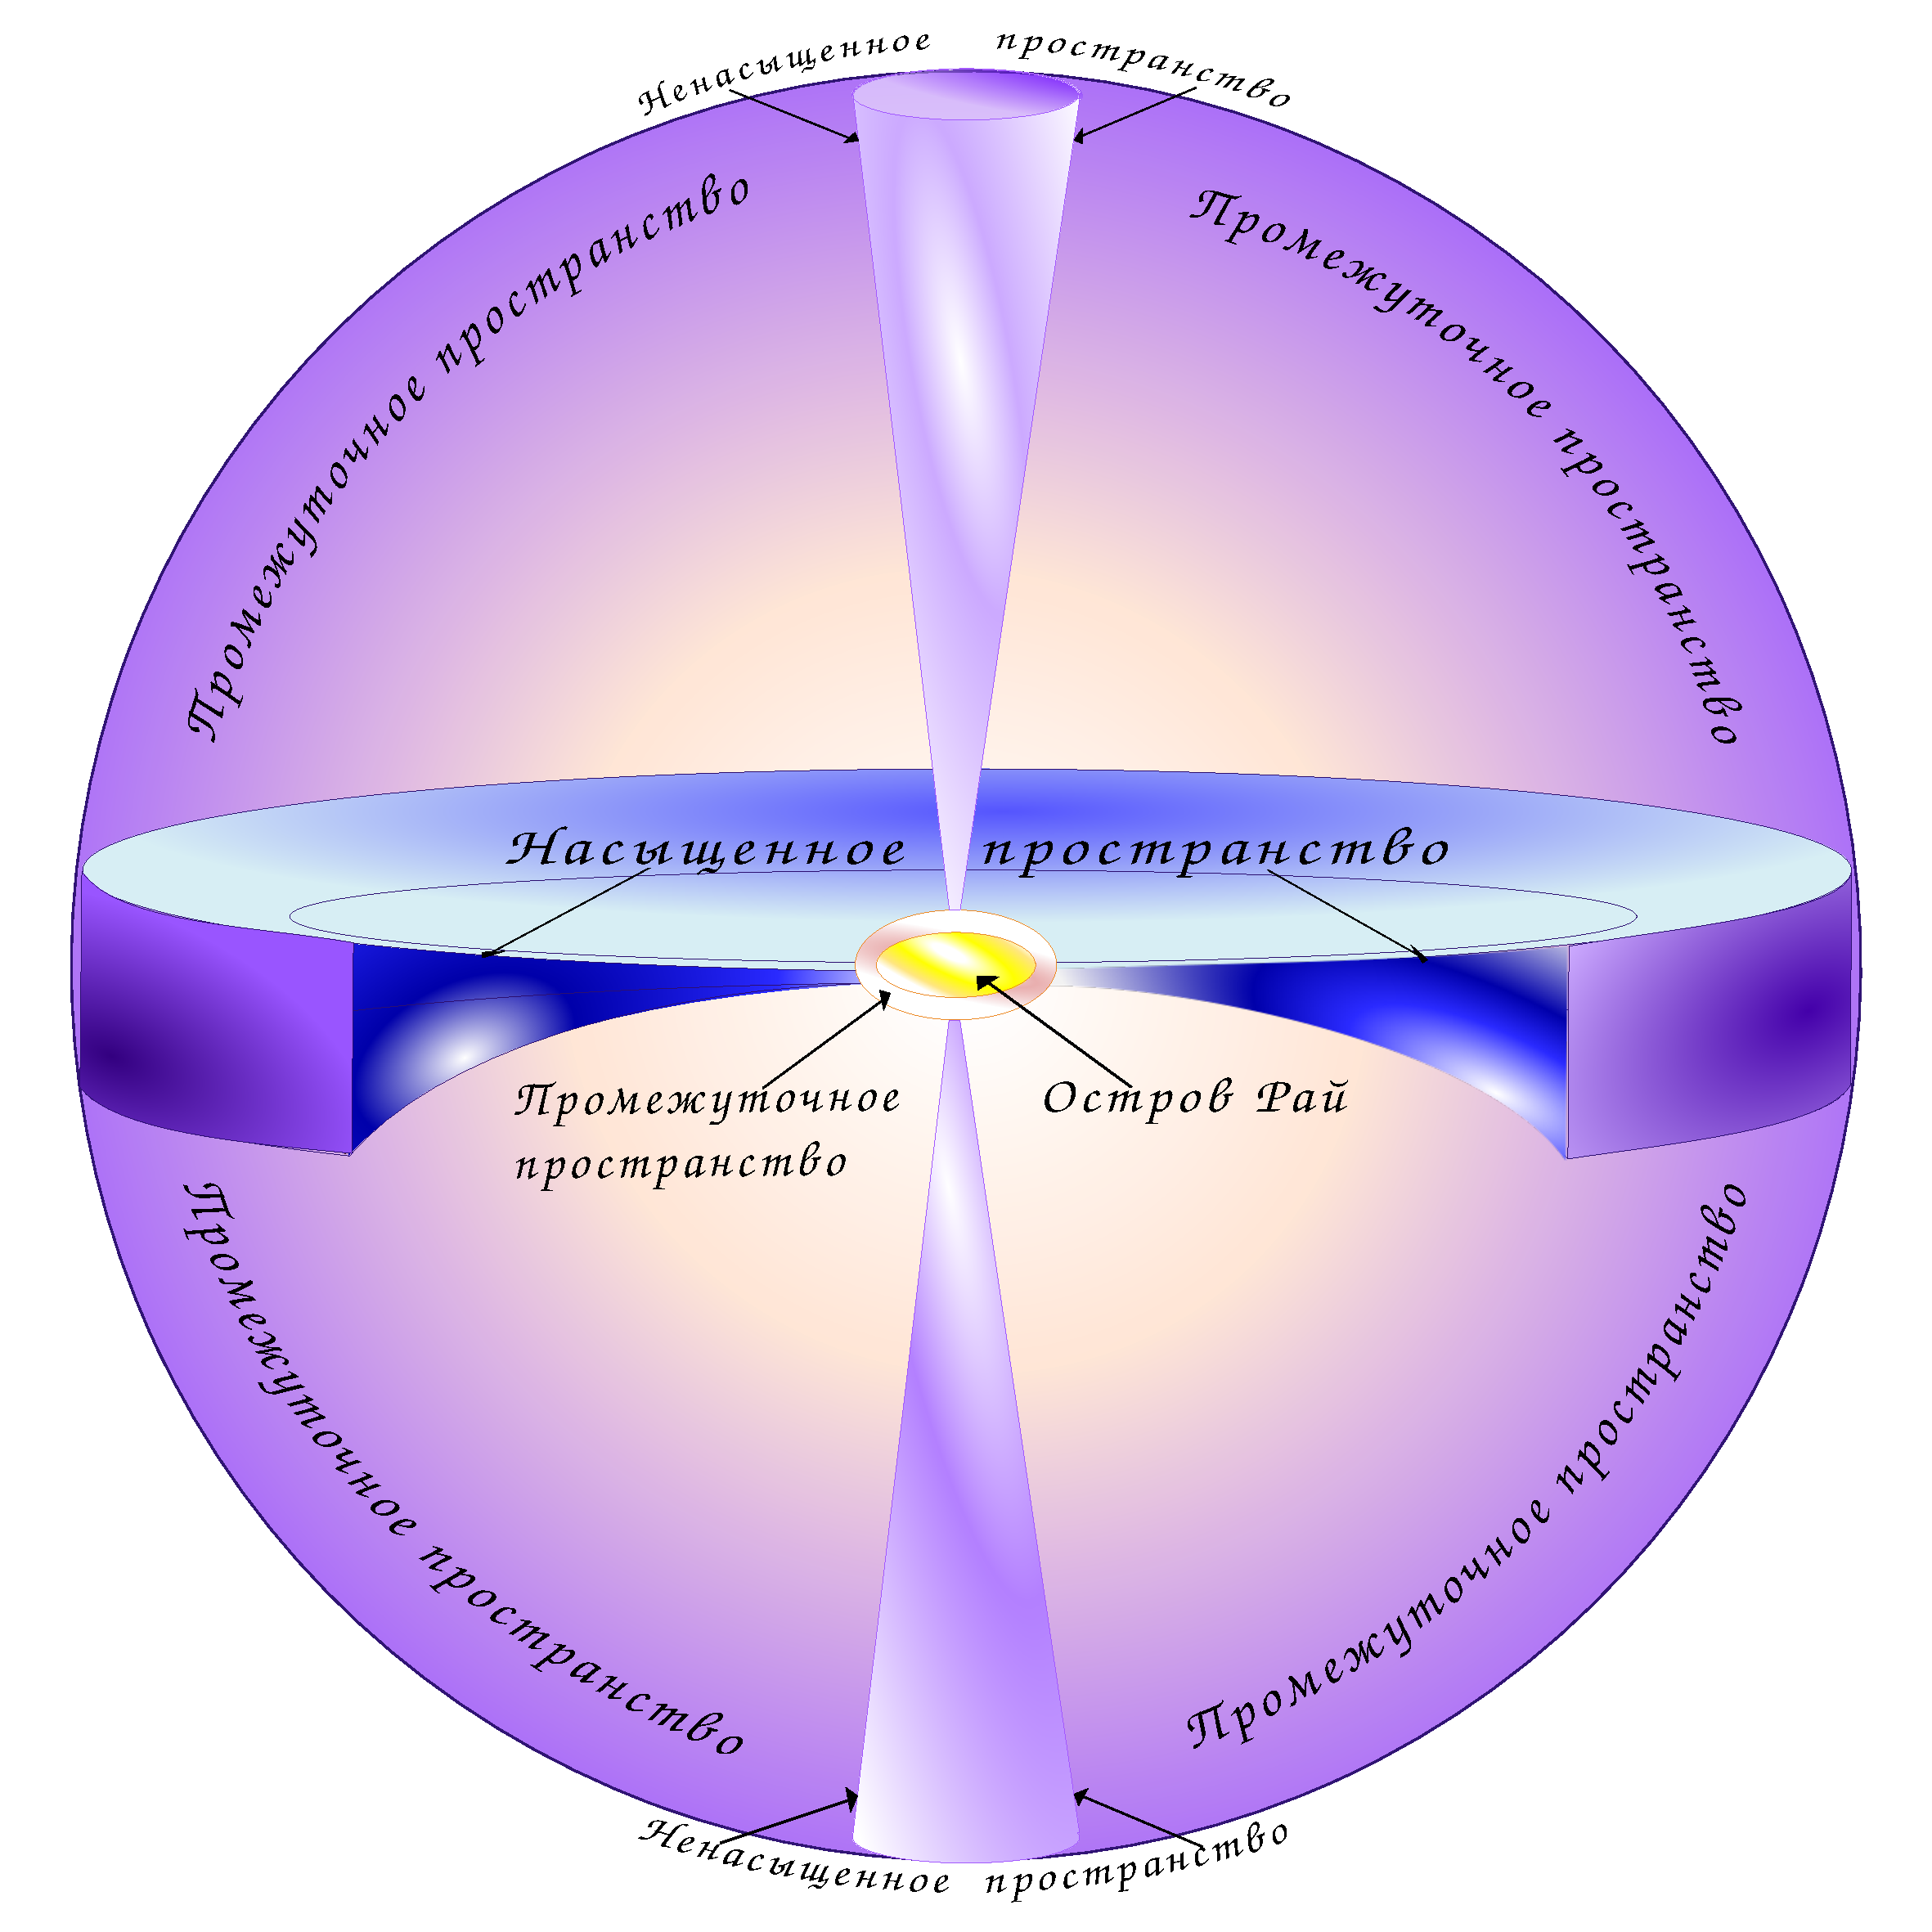
\includegraphics[width=0.99\columnwidth]{images/prostranstvo.pdf}\caption{Пространственные функции Рая}\end{figure}}
\vs p011 7:5 Если ты вообразишь себе конечную, но непостижимо огромную V\hyp{}образную плоскость, расположенную под прямым углом как к верхней, так и к нижней поверхностям Рая, и с вершиной, почти соприкасающейся с периферийным Раем, а затем представишь себе эту плоскость в эллиптическом обращении вокруг Рая, её вращение приблизительно очертит объём насыщенного пространства.
\vs p011 7:6 По отношению к любому заданному месту во вселенных существует верхний и нижний пределы горизонтального пространства. Если двигаться достаточно далеко под прямым углом к плоскости Орвонтона вверх или вниз, в конечном итоге можно достичь верхней или нижней границы насыщенного пространства. В пределах известных размеров главной вселенной эти пределы отдаляются всё дальше и дальше на всё б\'ольших и б\'ольших расстояниях от Рая; пространство сгущается, причём несколько быстрее, чем плоскость творения --- вселенные.
\vs p011 7:7 \pc Относительно спокойные зоны\fnst{В издании 1955 года слово <<зона>> в единственном числе.} между пространственными уровнями, такие как зона, отделяющая семь сверхвселенных от первого внешнего уровня пространства, представляют собой огромные эллиптические регионы спокойной пространственной деятельности. Эти зоны разделяют огромные галактики, которые в стройном шествии мчатся вокруг Рая. Можно представить себе первый внешний уровень пространства, где в настоящее время формируются бесчисленные вселенные, как гигантскую процессию галактик, обращающихся вокруг Рая, ограниченную сверху и снизу зонами покоя промежуточного пространства, и ограниченную на внутренней и внешней границах зонами относительно спокойного пространства.
\vs p011 7:8 Так пространственный уровень функционирует как эллиптическая область движения, со всех сторон окружённая относительной неподвижностью. Такие отношения движения и покоя составляют искривлённую пространственную траекторию уменьшённого сопротивления движению, по которой всегда следуют космическая сила и возникающая энергия в их вечном кружении вокруг Острова Рай.
\vs p011 7:9 Чередующиеся зоны главной вселенной в сочетании с чередующимся движением галактик по и против часовой стрелки являются фактором стабилизации физической гравитации, предназначенным предотвратить усиление гравитационного напряжения до точки разрушающих и рассеивающих процессов. Такое устройство оказывает антигравитационное влияние и действует как тормоз, гасящий опасные скорости.
\usection{ГРАВИТАЦИЯ РАЯ}
\vs p011 8:1 Неотвратимое гравитационное притяжение эффективно удерживает все миры всех вселенных всего пространства. Гравитация --- это всемогущие объятия физического присутствия Рая. Гравитация --- это всесильная нить, на которую нанизаны мерцающие звёзды, сияющие солнца и вращающиеся сферы, составляющие всеобщее физическое украшение вечного Бога, который есть всё, наполняет всё и в котором всё заключено.
\vs p011 8:2 Остров Рай --- это центр и фокальная точка абсолютной материальной гравитации, дополняемый тёмными гравитационными телами, окружающими Хавону, и уравновешиваемый верхним и нижним резервуарами пространства. Все известные излучения нижнего Рая неизменно и безошибочно откликаются на центральное гравитационное притяжение, действующее на бесконечные контуры эллиптических пространственных уровней главной вселенной. Каждая известная форма космической реальности обладает вековым изгибом, тенденцией круга, размахом огромного эллипса.
\vs p011 8:3 Пространство невосприимчиво к гравитации, но действует на неё как уравновешивающее средство. Без амортизирующей способности пространства взрывное действие сотрясало бы окружающие космические тела. Насыщенное пространство оказывает также антигравитационное воздействие на физическую, или линейную, гравитацию; пространство может фактически нейтрализовать такое действие гравитации, хотя оно не может замедлить его. Абсолютная гравитация --- это гравитация Рая. Локальная, или линейная, гравитация относится к электрической стадии энергии или материи; она действует в пределах центральной, сверх\hyp{} и внешних вселенных, --- везде, где произошла соответствующая материализация.
\vs p011 8:4 \pc Многочисленные формы космической силы, физической энергии, вселенской мощи и различные виды материализаций раскрывают три основные, хотя и не строго разделённые, стадии отклика на гравитацию Рая:
\vs p011 8:5 \li{1.}\bibemph{Догравитационные стадии (Сила)}. Это первый шаг в процессе индивидуации потенции пространства в формы предэнергии космической силы. Это состояние аналогично концепции изначальной силы\hyp{}заряда пространства, иногда называемого \bibemph{чистая энергия} или \bibemph{сегрегата}.
\vs p011 8:6 \li{2.}\bibemph{Гравитационные стадии (Энергия)}. Эта модификация силы\hyp{}заряда пространства вызвана действием Райских организаторов силы. Она сигнализирует появление энергетических систем, реагирующих на притяжение гравитации Рая. Эта возникающая энергия изначально нейтральна, но в результате дальнейших метаморфоз проявляет так называемые отрицательные и положительные качества. Мы называем эти стадии \bibemph{ультимата}.
\vs p011 8:7 \li{3.}\bibemph{Постгравитационные стадии (Вселенская мощь)}. На этой стадии энергия\hyp{}материя начинает отзываться на управление линейной гравитации. В центральной вселенной эти физические системы представляют собой тройственные организации, известные как \bibemph{триата}. Они являются сверхмощными материнскими системами творений времени и пространства. Физические системы сверхвселенных мобилизуются Управляющими Вселенской Мощью и их партнёрами. Эти материальные организации являются двойственными по строению и известны как \bibemph{гравита}. Тёмные гравитационные тела, окружающие Хавону, не являются ни триатой, ни гравитой, а сила их притяжения раскрывает обе формы физической гравитации: линейную и абсолютную.
\vs p011 8:8 \pc Потенция пространства не подвержена никаким гравитационным взаимодействиям. Этот изначальный дар Рая не является актуальным уровнем реальности, но он предшествует всем относительным функциональным недуховным реальностям --- всем проявлениям силы\hyp{}энергии и организации мощи и материи. Потенция пространства --- трудноопределимый термин. Он не означает чего\hyp{}либо предшествующего пространству; его значение должно передавать идею о потенциальных возможностях, существующих внутри самог\'о пространства. Приблизительно можно представить, что он включает все те абсолютные влияния и потенциалы, которые исходят из Рая и составляют пространственное присутствие Безусловного Абсолюта.
\vs p011 8:9 Рай --- это абсолютный источник и вечная фокальная точка всей энергии\hyp{}материи во вселенной вселенных. Безусловный Абсолют --- раскрыватель, регулятор и хранитель всего того, что имеет Рай в качестве своего источника и первопричины. Всеобщее присутствие Безусловного Абсолюта представляется эквивалентом концепции потенциальной бесконечности гравитационной протяжённости, упругого напряжения Райского присутствия. Эта концепция помогает нам понять тот факт, что всё тянется вовнутрь, к Раю. Иллюстрация грубая, но тем не менее полезная. Она также объясняет, почему гравитация всегда действует предпочтительно в плоскости, перпендикулярной массе\fnst{Как может быть \bibemph{плоскость} перпендикулярна \bibemph{массе?} Это всё равно, что сказать <<прямая, перпендикулярная апельсину>>. Тем не менее некоторые соображения теоретического и эмпирического характера могут пролить некоторый свет на эту загадку. Во\hyp{}первых, решение задачи двух тел, сводящееся, как известно, к движению точки приведённой массы в центральном силовом поле, показывает, что орбиты обоих тел находятся в одной плоскости, перпендикулярной вектору момента количества движения. В случае планет, обращающихся вокруг центральной звезды, это \bibemph{плоскость эклиптики}. При разгоне транспортного серафима до скорости света (и более) движение происходит в направлении, \bibemph{перпендикулярном} плоскости эклиптики. Возможно, такой манёвр является энергетически выгодным для серафима и имеет какое\hyp{}то отношение к упомянутому в тексте факту предпочтительного действия гравитации в определённой плоскости.}, --- феномен, указывающий на различия в размерах Рая и окружающих его творений.
\usection{УНИКАЛЬНОСТЬ РАЯ}
\vs p011 9:1 Рай уникален тем, что является областью изначального происхождения и конечной целью предназначения всех духовных личностей. Хотя верно, что не все низшие духовные существа локальных вселенных имеют непосредственным предназначением Рай, всё же Рай остаётся желанной целью всех сверхматериальных личностей.
\vs p011 9:2 \pc Рай --- это географический центр бесконечности; это не часть всеобщего творения, и даже не реальная часть вечной вселенной Хавоны. Обычно мы относим центральный Остров к божественной вселенной, но на самом деле это не так. Рай --- это вечное и исключительное существование.
\vs p011 9:3 \pc В вечности прошлого, когда Всеобщий Отец дал бесконечное личностное выражение своего духовного <<я>> в существе Вечного Сына, одновременно он раскрыл бесконечный потенциал своего неличностного <<я>> в виде Рая. Неличностный и недуховный Рай представляется неизбежным отражением воли Отца и актом, увековечившим Изначального Сына. Таким образом, Отец спроецировал реальность в двух актуальных фазах: личностной и неличностной, духовной и недуховной. Напряжение между ними перед лицом воли к действию со стороны Отца и Сына дало существование Совместному Вершителю и центральной вселенной материальных миров и духовных существ.
\vs p011 9:4 Когда реальность разделена на личностную и неличностную (Вечный Сын и Рай), вряд ли уместно называть неличностное <<Божеством>> без каких\hyp{}либо оговорок. Энергетические и материальные последствия действий Божества вряд ли можно назвать Божеством. Божество может служить причиной многого того, что не является Божеством, и Рай --- это не Божество; не обладает Рай и сознанием в любом возможном понимании этого термина смертным человеком.
\vs p011 9:5 \pc Рай не является первопричиной какого\hyp{}либо существа или живого организма; это не создатель. Личность и отношения между разумом\hyp{}духом могут \bibemph{передаваться,} но образец --- нет. Образцы никогда не являются отражениями; они могут быть представлены копиями, репродукциями. Рай --- это абсолют образцов; Хавона --- демонстрация этих потенциалов в актуальности.
\vs p011 9:6 \pc Резиденция Бога --- центральная и вечная, славная и идеальная. Его дом --- прекрасный образец для всех столичных миров вселенных; и центральная вселенная его непосредственного обитания служит образцом для всех вселенных в их идеалах, организации и конечном предназначении.
\vs p011 9:7 Рай --- это всеобщий центр всей личностной деятельности и источник\hyp{}центр всех проявлений силы\hyp{}пространства и энергии. Всё, что было, есть и ещё должно быть, произошло, происходит и будет происходить из этой центральной обители вечных Богов. Рай --- это центр всего творения, источник всех энергий и место изначального происхождения всех личностей.
\vs p011 9:8 \pc В конечном итоге самое важное для смертных в вечном Раю --- это тот факт, что эта совершенная обитель Всеобщего Отца есть реальная и далёкая цель бессмертных душ смертных и материальных сынов Бога, восходящих созданий эволюционных миров времени и пространства. Каждый Богопознавший смертный, посвятивший себя делу исполнения воли Отца, уже вступил на долгий, долгий Райский путь стремления к божественности и достижения совершенства. И когда такое существо животного происхождения предстаёт, как предстают сейчас бесчисленные множества, перед Богами в Раю, поднявшись из скромных сфер пространства, такое достижение представляет реальность духовной трансформации, граничащей с пределами верховности.
\vsetoff
\vs p011 9:9 [Представлено Совершенствователем Мудрости, уполномоченным для этих действий От Века Древними Уверсы.]
\quizlink
